\clearpage
\crshead{ГЛАВА 2. Анализ физических источников энтропии и их применение в
генераторах истинно случайных последовательностей}

\crssubhead{2.1. Электронные источники шума}

При проектировании интегральных схем шум неизбежен и нежелателен. Однако
в физических ГИСП улавливание и усиление непредсказуемых и
неконтролируемых человеком источников шума являются основополагающими
принципами. Для хорошей модели источника энтропии сам источник должен
представлять собой белый шум с гауссовым распределением. Таким образом,
качество источника энтропии напрямую зависит от наблюдаемых свойств
генерируемого им шума.

Выделим и проанализируем 4 основных вида электронных источников энтропии
пригодных для разработки ГСП:

\begin{enumerate}
\def\labelenumi{\arabic{enumi}.}
\item
  Тепловой шум
\item
  Дробовой шум
\item
  Лавинный шум
\item
  Мерцающий шум
\end{enumerate}

\textbf{Тепловой шум}, также называемый шумом Джонсона-Найквиста или
термическим шумом -- это электронный шум, возникающий в результате
теплового возбуждения носителей заряда, обычно электронов, в
электрическом проводнике. Этот вид шума возникает в любом резисторе с
ненулевой температурой и имеет строго физическую природу, основанную на
хаотичном тепловом движении электронов. Белый гауссов шум, генерируемый
резистором за счёт тепловой агитации носителей заряда впервые был описан
в работах Джона Б. Джонсона и Гарри Найквиста в 1928 году.

Среднеквадратичное напряжение теплового шума в заданной полосе (согласно
формуле Найквиста){[}11{]}{[}13{]}:

\[\overline{e_{t}^{2}} = 4kTR\mathrm{\Delta}f\]

где:

\begin{quote}
\(\overline{e_{t}^{2}}\) -- cреднеквадратичное напряжение шума,

\emph{k} ≈ 1.38×10\textsuperscript{23} Дж/К~-- постоянная Больцмана,

\emph{T} -- абсолютная температура резистора в кельвинах,

\emph{R} -- сопротивление в омах,

\(\mathrm{\Delta}f\) = \emph{f\textsubscript{upper}} --
\emph{f\textsubscript{lower }}-- выбранная для измерения полоса частот
\end{quote}

Спектральная плотность напряжения такого шума задаётся формулой{[}11{]}:

\[S_{f} = 4kTR\frac{hf}{kT}(exp{\frac{hf}{kT} - 1)}^{- 1}\]

где:

\begin{quote}
\emph{h} ≈ 6,626×10\textsuperscript{−34}~Дж*с \emph{--} постоянная
Планка

\(S_{f}\) -- спектральная плотность (В\textsuperscript{2}*с)
\end{quote}

График зависимости спектральной плотности от частоты при комнатной
температуре представлен на рисунке 3.

\begin{center}\begin{minipage}{\linewidth}\centering
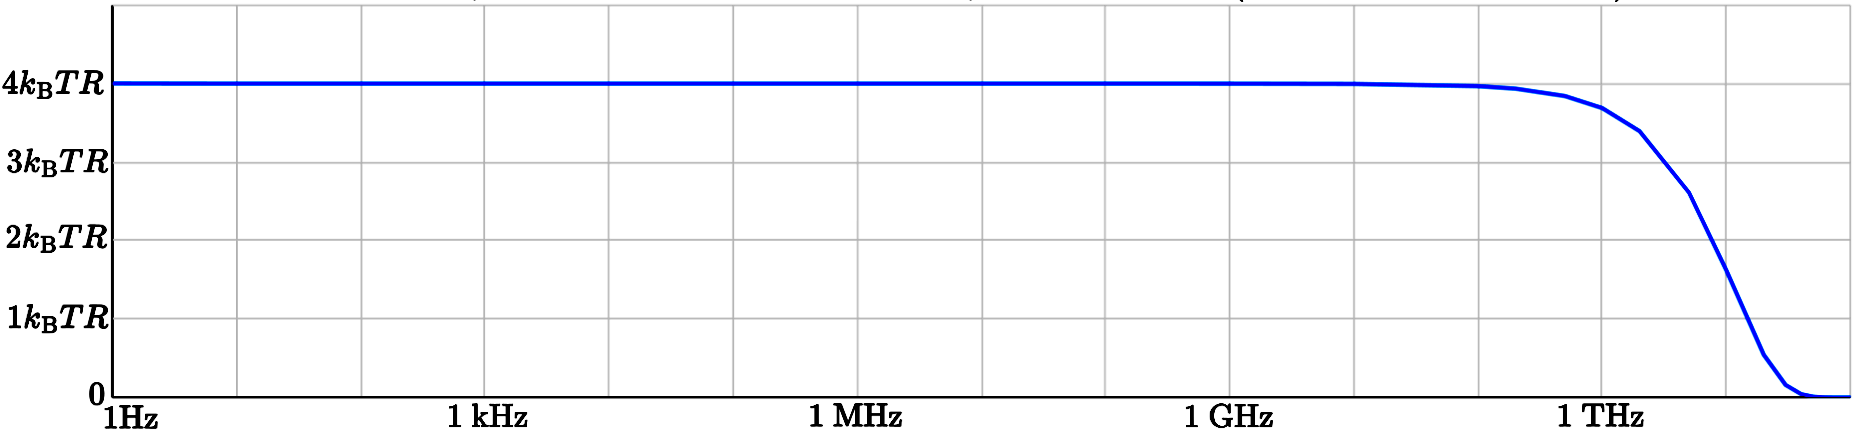
\includegraphics[width=\linewidth,keepaspectratio]{pandoc_media/media/image3.png}

Рисунок 3.
\end{minipage}\end{center}

Для области соответствующей условию:

\[\frac{hf}{kT} \ll 1\]

Иными словами, для частот, значительно меньших, чем

\[f_{\max} \approx \frac{kT}{h}\]

\[(f_{\max} \approx 6 \times 10^{12}Гц\ при\ 300К)\]

Можем считать спектральную плотность постоянной независимой от
частоты{[}11{]}:

\[S_{f} = \frac{\overline{e_{t}^{2}}}{\mathrm{\Delta}f} = 4kTR\]

Эта спектральная плотность не зависит от частоты (в диапазоне до
десятков гигагерц), поэтому шум считается белым.

Чтобы использовать этот шум в ГИСП, необходимо выполнить несколько
этапов:

1. Формирование сигнала. Электрическое напряжение, наведённое тепловым
шумом на резисторе, усиливается с помощью малошумящего операционного
усилителя.

2. Ограничение полосы частот. Сигнал пропускается через полосовой
(bandpass) фильтр, чтобы исключить внешние помехи и отсечь побочные
частоты.

3. Оцифровка. Полученный аналоговый сигнал дискретизируется и квантуется
с помощью АЦП (аналогово-цифрового преобразователя). Результатом
является последовательность значений, например 8- или 12-битных.

4. Преобразование в случайные биты. Используется постобработка:
вырезание младших битов, хэш-функции или экстракция с помощью
алгоритмов, таких как Von Neumann extractor или Hash-based extractor,
чтобы устранить корреляции и повысить энтропию.

Количество энтропии, генерируемое за единицу времени, зависит от ширины
полосы Δ\emph{f}, температуры \emph{T}, сопротивления \emph{R}, точности
АЦП и скорости дискретизации. Важно понимать, что после АЦП не все биты
одинаково случайны: старшие биты могут быть предсказуемы, особенно при
низком уровне шума. Поэтому чаще всего используются младшие биты, иногда
с дополнительной энтропийной компрессией.

Преимущества использования теплового шума в роли источника энтропии в
ГИСП:

\begin{itemize}
\item
  Высокая надёжность и физическая непредсказуемость.
\item
  Отсутствие квантовых эффектов (при правильно настроенном полосовом
  фильтре).
\end{itemize}

Недостатки:

\begin{itemize}
\item
  Уязвимость к внешним электромагнитным помехам.
\item
  Необходимость сложной постобработки для получения равномерного
  распределения.
\item
  Необходимость температурной стабилизации для поддержания стабильного
  уровня шума.
\end{itemize}

Блок-схема проектирования ГИСП на основе теплового шума может выглядеть
следующим образом (рисунок 4):

\begin{center}\begin{minipage}{\linewidth}\centering
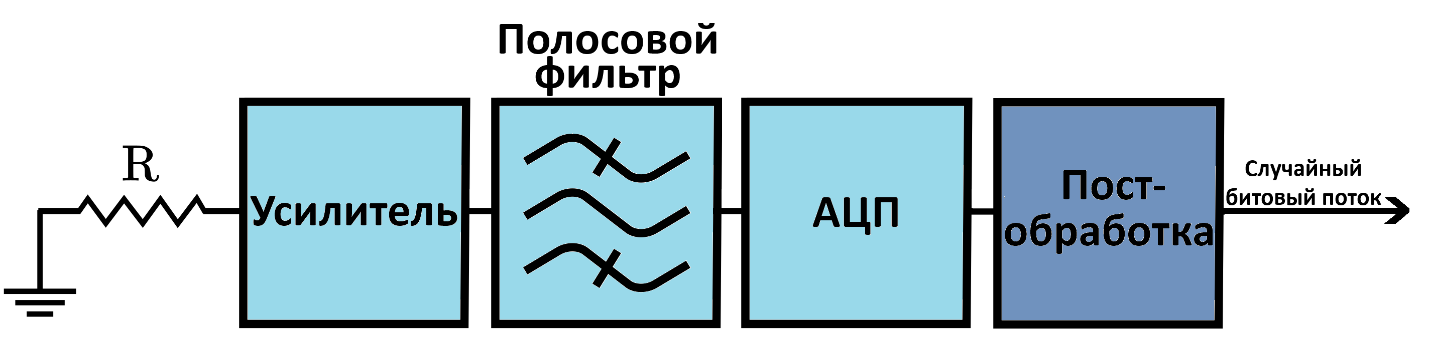
\includegraphics[width=\linewidth,keepaspectratio]{pandoc_media/media/image4.png}

Рисунок 4
\end{minipage}\end{center}

Изучая в 1918 году тепловой шум с использованием теорий Эйнштейна,
Уолтер Шоттки экспериментально обнаружил другой вид шума -- дробовой
шум.

\textbf{Дробовой шум} (shot noise\emph{,} шум Пуассона) -- это
электронный шум, связанный с дискретной (квантованной) природой
электрического тока. Он возникает из-за того, что заряд переносится не
непрерывно, а в виде отдельных частиц -- электронов. Когда электроны
пересекают потенциальный барьер (например, в p-n переходе, вакуумном
диоде, туннельном переходе и т.д.), они делают это случайным образом,
независимо друг от друга, что приводит к флуктуациям тока, даже если
средний ток постоянен. Термин «дробовой шум» (а также дробовой эффект)
возник в связи с тем, что благодаря ему в громкоговорителе, подключённом
к выходу усилителя или радиоприёмника, появляется акустический шум,
воспринимаемый ухом как напоминающий шум сыплющихся дробинок.

Впервые дробовой шум был теоретически описан Уолтером Шоттки в 1918
году, когда он исследовал шумовые характеристики вакуумных ламп.

Среднеквадратичное значение тока шума Шоттки за интервал времени
определяется как{[}12{]}{[}13{]}:

\[\overline{i_{s}^{2}} = 2qI\Delta f\]

где:

\begin{quote}
\(\overline{i_{s}^{2}}\)\hspace{0pt}\hspace{0pt} -- дисперсия тока шума,

\emph{q} ≈ 1.6×10\textsuperscript{−19} Кл --- заряд электрона,

\emph{I} -- средний ток (А),

Δ\emph{f} -- ширина полосы частот (Гц).
\end{quote}

Спектральная плотность дробового шума также постоянна во всём частотном
диапазоне и задаётся формулой{[}11{]}:

\[S_{I}(f) = 2qI\]

В отличие от теплового шума, который зависит от температуры, дробовой
шум не зависит от температуры, но зависит от среднего тока I.

Дробовой шум наблюдается только в условиях, когда поток зарядов не
является непрерывным:

\begin{itemize}
\item
  в вакуумных диодах,
\item
  в фотоэлектронных приборах,
\item
  в туннельных диодах,
\item
  в слабонасыщенных p-n переходах,
\item
  в фотодетекторах (где ток создаётся фотонами, а не внешним
  напряжением).
\end{itemize}

В металлических проводниках дробовой шум обычно подавлен за счёт эффекта
выравнивания потенциала и действия Паули, поэтому там преобладает
тепловой шум.

Чтобы использовать дробовой шум в генераторах истинных случайных чисел,
реализуется следующая схема:

1. Формирование тока. Используется p-n переход или фотодиод в режиме
слаботекущего тока (порядка наноампер --- микроампер). При этом
создаётся ток, насыщенный дробовым шумом.

2. Преобразование в напряжение. Ток преобразуется в напряжение с помощью
токозависимого усилителя или прецизионного резистора.

3. Усиление. Сигнал усиливается, при этом важно сохранить соотношение
сигнал/шум и не вносить дополнительный шум от усилителя.

4. Ограничение полосы частот. Подача на полосовой фильтр для выделения
нужного частотного диапазона.

5. Оцифровка. Сигнал поступает на АЦП. Аналогично тепловому шуму,
оцифрованный сигнал содержит "сырые" данные.

6. Постобработка. Применяются алгоритмы, повышающие качество случайных
битов --- например, хэширование или алгоритм фон Неймана.

Как и тепловой шум, дробовой шум имеет равномерную спектральную
плотность, и его можно считать белым в широком диапазоне частот.

Преимущества дробового шума как источника энтропии:

\begin{itemize}
\item
  Основан на фундаментальной квантовой природе тока (дискретность
  зарядов).
\item
  Относительно простая реализация при наличии фотодиода и
  соответствующего усилителя.
\item
  Хорошая устойчивость к температурным флуктуациям.
\end{itemize}

Недостатки:

\begin{itemize}
\item
  Требует стабильного и строго контролируемого источника тока.
\item
  Очень малые токи дают слабый уровень шума, что требует высокоточного
  усиления.
\item
  Чувствительность к освещению (в случае фотодиодов) и к
  электромагнитным помехам.
\end{itemize}

Условная схема ГИСП на основе дробового шума может быть представлена в
виде цепочки модулей (рисунок 5).

\begin{center}\begin{minipage}{\linewidth}\centering
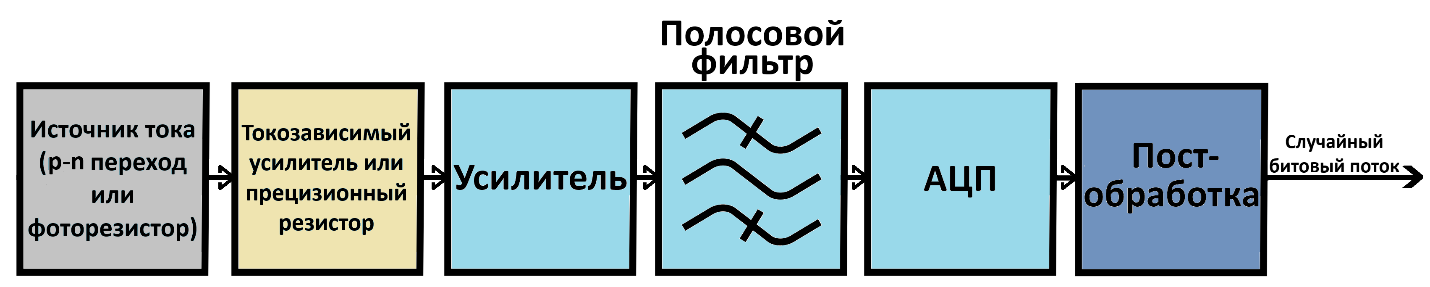
\includegraphics[width=\linewidth,keepaspectratio]{pandoc_media/media/image5.png}

Рисунок 5
\end{minipage}\end{center}

\textbf{Лавинный шум} --- это разновидность дробового шума, возникающая
в полупроводниковых приборах с внутренним усилением, таких как лавинные
фотодиоды (APD, avalanche photodiodes), лавинные транзисторы,
стабилитроны или p--n переходы при пробое. Он обусловлен стохастическим
характером процесса лавинной генерации носителей, при котором один
носитель может возбуждать несколько новых носителей через ударную
ионизацию.

Когда напряжение на p--n переходе превышает определённый порог,
начинается ударная ионизация: свободные электроны, ускоряясь
электрическим полем, ионизируют атомы кристаллической решётки, создавая
новые пары электрон - дырка. Этот процесс накапливается лавинообразно и
приводит к внутреннему усилению сигнала. Поскольку число новых носителей
в каждой лавине случайно, процесс сопровождается флуктуациями, т.е.
шумом.

При учёте коэффициента внутреннего усиления M и коэффициента избыточного
шума F, спектральная плотность тока лавинного шума задаётся{[}11{]}:

\[S_{I}(f) = 2qIM^{2}F\]

где:

\begin{quote}
\(S_{I}(f)\) -- спектральная плотность тока, {[}А²/Гц{]},

\emph{q} ≈ 1,6×10\textsuperscript{−19} Кл -- заряд электрона,

\emph{I} -- средний фототок без усиления, {[}А{]},

\emph{M} -- коэффициент лавинного усиления,

\emph{F} -- коэффициент избыточного шума, зависящий от технологии
(например, \emph{F} ≈ \emph{M} при равных вероятностях ионизации
электронов и дырок).
\end{quote}

При моделировании с учётом разных ионизационных вероятностей для
электронов и дырок (k) используется приближённая формула{[}11{]}:

\[F(M) = kM + \left. \ \left( 2 - \frac{1}{M} \right.\  \right)(1 - k)\]

где: \emph{k} ∈ {[}0,1{]} -- отношение коэффициентов ионизации дырок к
электронам (для кремния \emph{k} ≪ 1, для арсенида галлия -- \emph{k} ≈
0.4).

Для построения генераторов случайных чисел на основе лавинного шума
применяются лавинные фотодиоды, работающие в режиме ниже или около
пробоя. Шум усиливается, фильтруется, оцифровывается и проходит
постобработку, как и в системах на тепловом или дробовом шуме.
Преимущество лавинного шума -- более высокая амплитуда флуктуаций, что
может повысить отношение сигнал/шум.

Преимущества:

\begin{itemize}
\item
  Очень высокий уровень шума даже при малых токах.
\item
  Возможность построения компактных источников энтропии.
\item
  Хорошо подходит для светочувствительных систем.
\end{itemize}

Недостатки:

\begin{itemize}
\item
  Сильная температурная зависимость.
\item
  Необходимость прецизионного контроля напряжения, чтобы избежать
  перехода в режим пробоя.
\item
  Лавинные процессы могут вызывать деградацию прибора со временем.
\end{itemize}

\textbf{Мерцающий шум}, также известный как шум с обратной
пропорциональностью к частоте (англ. flicker noise или \emph{1/f}
noise), представляет собой тип низкочастотного шума, который наблюдается
в широком классе электронных компонентов --- в первую очередь в
МОП-транзисторах, резисторах и других полупроводниковых приборах. Его
характерной особенностью является спектральная плотность мощности,
обратно пропорциональная частоте: \(S(f) \propto \frac{1}{f^{\gamma}}\),
где~γ ≈ 1

Физическая природа 1/f шума до конца не установлена, но в
МОП-транзисторах основной вклад в него дают следующие механизмы:

\begin{itemize}
\item
  Флуктуации числа носителей заряда (Carrier Number Fluctuation):
\end{itemize}

Происходят за счёт захвата и высвобождения носителей в ловушках на
границе оксид-полупроводник.

\begin{itemize}
\item
  Флуктуации подвижности носителей (Carrier Mobility Fluctuation):
\end{itemize}

Возникают из-за нестационарности рассеяния носителей, например, за счёт
изменения локального электрического поля.

\begin{itemize}
\item
  Комбинация CNF и CMF может приводить к коррелированным
\end{itemize}

эффектам, усиливая спектральную плотность шума

Спектральная плотность напряжения 1/f шума обычно приближённо выражается
так{[}12{]}:

\[S_{V}(f) = \frac{K}{C_{ox}^{2}WL}\frac{1}{f}\]

где:

\begin{quote}
\emph{K} --- эмпирический коэффициент, зависящий от технологического
процесса,

\(C_{ox}\) --- ёмкость оксида затвора на единицу площади,

\emph{W} и \emph{L} --- ширина и длина канала транзистора
соответственно,

\emph{f} --- частота.
\end{quote}

Таким образом, шум усиливается при уменьшении размеров транзистора,
особенно при переходе к нанометровым техпроцессам.

В сравнении с тепловым шумом, обладающем постоянной спектральной
плотностью (\(S(f) = const\)), 1/f шум, наоборот, убывает с увеличением
частоты и доминирует на низких частотах. Существует частота пересечения
(так называемая \emph{угловая частота}), выше которой 1/f шум становится
слабее теплового шума. Ниже этой частоты он начинает преобладать.

В генераторах случайных чисел (ГСЧ) 1/f шум может вызывать корреляции
между выходными битами, особенно при недостаточной скорости выборки. Это
делает его менее эффективным для генераторов, работающих на высоких
частотах. Формально, выходной сигнал ГСЧ может быть подвержен
автокорреляции:

\(Corr(X_{t},X_{t + \tau}) > 0\) при~малых~τ

где \(X_{t}\) -- выходной бит в момент времени t.

Хотя мерцающий шум сам по себе не является идеальным источником
энтропии, при правильной архитектуре он может служить источником
энтропии для низкоскоростных TRNG или добавочным источником к тепловому
или дробовому шуму.

\begin{quote}
\crssubhead{2.2. Оптические и квантовые источники}
\end{quote}

Квантовая физика лежит в основе современного понимания устройства
материи. Одной из ключевых особенностей квантовых процессов является их
фундаментальная недетерминированность. Это означает, что даже при точном
знании начальных условий результат квантового измерения нельзя
предсказать однозначно. Именно это делает квантовые явления естественным
и надежным источником истинной случайности.

Классические генераторы случайных последовательностей (ГСП), в отличие
от квантовых, работают на основе детерминированных физических процессов.
Их "случайность" обусловлена только недостатком информации о начальных
параметрах системы, а потому при теоретически полной информации
поведение таких систем становится предсказуемым. В связи с этим только
квантовые ГСП можно строго научно обосновать как источники истинной
энтропии.

Квантовые генераторы случайных чисел (КГСЧ) используют одиночный
квантовый эффект, воспроизводимый в идентичных начальных условиях.
Несмотря на это, каждый эксперимент даёт непредсказуемый результат --- в
полном соответствии с законами квантовой механики.

В основе большинства КГСЧ лежит работа с кубитами --- квантовыми
аналогами битов, которые могут находиться в двух состояниях: (0) и (1),
либо в их суперпозиции. Примерами физических реализаций кубитов являются
спин электрона или поляризация фотона. При измерении кубита он «падает»
в одно из этих состояний, а результат измерения непредсказуем и
подчиняется вероятностному закону.

Система из L кубитов имеет 2\textsuperscript{L} возможных независимых
состояний. Это позволяет квантовым устройствам выполнять параллельные
вычисления и использовать квантовую суперпозицию для генерации случайных
битов.

Пример: генерация с помощью поляризованных фотонов

Часто для создания КГСЧ применяют фотоны. Их удобно создавать,
направлять и детектировать. Одна из простейших схем генерации случайных
битов заключается в пропускании фотона с круговой поляризацией через
светоделительную пластину. Она разделяет фотон на два возможных пути --
горизонтальный и вертикальный -- с равной вероятностью. Направление
выхода фотона (влево или вправо), фиксируемое соответствующим
детектором, интерпретируется как логический 0 или 1 (Рисунок 6){[}3{]}.
Даже при неизменной установке и начальных условиях результат
эксперимента каждый раз может быть разным, поскольку выбор пути фотоном
является по своей природе квантово-случайным.

\begin{center}\begin{minipage}{\linewidth}\centering
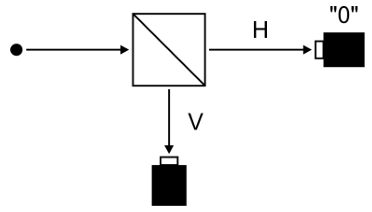
\includegraphics[width=\linewidth,keepaspectratio]{pandoc_media/media/image6.png}

Рисунок 6
\end{minipage}\end{center}

Физическая случайность при использовании оптических систем основана на
фундаментально вероятностной природе некоторых квантовых процессов, в
которых фотоны участвуют. Основными механизмами получения энтропии в
оптических квантовых генераторах являются спонтанное излучение,
расщепление пучка света и измерение флуктуаций оптического поля.

Существует также подход, при котором фотонные генераторы используют
временную характеристику событий -- например, измерение интервалов между
спонтанными выбросами фотонов лазером. Такие схемы основаны на временном
принципе, противоположном пространственному, где случайность кодируется
не в месте попадания фотона, а во времени его детектирования.

В ряде решений применяется метод регистрации квантовых флуктуаций
вакуумного поля с помощью высокочувствительных детекторов, таких как
гомодинные или гетеродинные схемы. Эти системы позволяют считывать
непрерывные шумовые сигналы, содержащие истинную квантовую энтропию, и
далее оцифровывать их для получения случайных битов.

Следует отметить, что оптические схемы обладают высокой
производительностью, а некоторые современные ГИСП на основе фотонов
достигают скоростей генерации десятков гигабит в секунду. В то же время
существует ряд практических ограничений. Несмотря на высокую степень
случайности, реальная реализация КГСЧ сталкивается с рядом технических
проблем:

1. Неидеальность компонентов: расщепление пучка может быть не совсем
симметричным; детекторы могут иметь разную эффективность.

2. Старение и температурные сдвиги: с течением времени свойства
оптических и электронных компонентов могут изменяться, нарушая
равновероятность выходных состояний.

3. Корреляции между битами: вызваны, например, временем восстановления
фотонного детектора, приводят к появлению зависимостей между
результатами последовательных измерений.

Для устранения этих недостатков применяется калибровка оборудования,
схемы с одним фотонным детектором и, при необходимости, постобработка
данных, которая снижает уровень корреляций до допустимого значения.

Особое внимание уделим радиоактивному распаду в качестве источника
энтропии. Радиоактивный распад является квантовомеханическим процессом,
происходящим самопроизвольно в нестабильных атомных ядрах. Вероятность
распада за бесконечно малый промежуток времени dt описывается
экспоненциальным законом:

\(P(t) = \lambda e^{- \lambda t}\),

где:

\begin{quote}
\emph{t} -- время, прошедшее с последнего распада,

\emph{λ} -- постоянная распада, связанная с периодом полураспада
\(T_{\frac{1}{2}}\)\hspace{0pt} через отношение
\(\lambda = \frac{ln2}{T_{\frac{1}{2}}}\)
\end{quote}

Величина t носит истинно случайный характер в пределах законов квантовой
механики. Это означает, что даже при полной информации об окружающей
среде невозможно точно предсказать момент следующего распада конкретного
атома.

Таким образом, временные интервалы между последовательными актами
радиоактивного распада представляют собой случайную величину с хорошо
описанной теоретической моделью.

Типичная реализация состоит из следующих компонентов:

\begin{enumerate}
\def\labelenumi{\arabic{enumi}.}
\item
  Радиоактивный изотоп с безопасной активностью (например, америций-241
  или стронций-90).
\item
  Детектор ионизирующего излучения -- например, счётчик Гейгера-Мюллера,
  кремниевый фотодиод или сцинтиллятор.
\item
  Схема счёта времени между детекциями событий (высокоточный таймер,
  например, с частотой 1--100 МГц).
\item
  Алгоритм дискретизации времени в битовые значения.
\end{enumerate}

Пусть последовательность времён регистрации событий обозначена как
\(\{ t_{1},t_{2},\ldots,t_{n}\}\). Тогда

\[\Delta t_{i} = t_{i} - t_{i - 1}\]

представляют собой независимые и экспоненциально распределённые
величины. Эти значения могут быть использованы как вход в функцию
дискретизации, например:

\begin{quote}
Младшие k битов \(\Delta t_{i}\)\hspace{0pt} используются как случайный
битовый поток.

Или применяется функция:

\[x_{i} = \left\{ \begin{array}{r}
1,\ \ если\ \Delta t_{i} > \tau \\
0,\ \ если\ \Delta ti \leq \tau
\end{array} \right.\ \]
\end{quote}

где τ -- эмпирически выбранный порог, обеспечивающий равновероятность 0
и 1.

Для устранения возможной остаточной корреляции и аппаратных искажений
применяются криптографически стойкие экстракторы энтропии, такие как:
хэш-функции (SHA-2, BLAKE2), метод фон Неймана (Von Neumann debiasing).

Несмотря на достаточно весомое количество преимуществ такой реализации,
квантовые ГИСП на основе радиоактивного распада имеют ряд ограничений и
проблем, наиболее значительные из которых:

\begin{itemize}
\item
  Ограниченная скорость генерации (≤10\textsuperscript{4} событий в
  секунду для безопасных изотопов).
\item
  Аппаратная сложность и стоимость, включая защиту от ионизирующего
  излучения.
\item
  Юридические и нормативные ограничения на использование радиоактивных
  веществ (например, требования Росатома или IAEA).
\item
  Необходимость калибровки и тестирования детекторов, учитывая старение,
  температурную нестабильность и возможные ложные срабатывания.
\end{itemize}

\crssubhead{2.3. Механические и акустические источники}

Помимо квантовых и оптических методов генерации случайных чисел, в ряде
практических приложений используются механические и акустические
источники энтропии. Эти методы опираются на макроскопические процессы,
которые, несмотря на свою классическую природу, обладают высокой
чувствительностью к начальному состоянию и внешним возмущениям, что
делает их полезными в качестве дополнительных или вспомогательных
компонентов в системах генерации случайных последовательностей.

\textbf{Механические} системы используются в генераторах случайных чисел
уже десятилетия. Одним из простейших исторических примеров является
механический бросок кости или вращение рулетки. В современных
электронных системах механические элементы могут использоваться более
технологично -- например, в виде микроэлектромеханических систем (MEMS),
вибрационных датчиков или гироскопов.

Случайность в таких системах формируется за счёт хаотического характера
движения, вызванного микроскопическими флуктуациями, вибрациями,
трением, турбулентными потоками воздуха и другими стохастическими
процессами. В случае MEMS-устройств генерация энтропии может
происходить, например, при считывании отклонений подвижных элементов от
их положения равновесия.

Однако стоит учитывать, что механические источники подвержены износу,
старению, температурным деформациям, а также могут демонстрировать
ограниченный спектр случайных состояний, что требует дополнительной
обработки данных и контроля качества выходной последовательности.

\textbf{Акустические} методы используют шумы, возникающие при вибрации
объектов, прохождении звуковых волн через различные среды или при работе
механических систем. В качестве источника энтропии может применяться
электронное считывание акустического шума, например, с микрофонов или
пьезоэлектрических датчиков.

Шумы окружающей среды, звуковые помехи в помещениях, тепловые флуктуации
в материалах -- всё это создаёт уникальные и сложно моделируемые
сигналы, которые при должной обработке могут использоваться для
генерации случайных битов. Часто в таких генераторах реализуется схема с
усилением слабого акустического сигнала, его последующей оцифровкой и
выделением энтропии путём анализа амплитудных и спектральных
характеристик.

Основная особенность механических и акустических источников состоит в
том, что они относятся к классическим стохастическим системам, где
случайность возникает не из-за фундаментальной неопределённости (как в
квантовых системах), а в результате сложности и непредсказуемости
начальных условий и чувствительности к внешним воздействиям.

Поэтому такие генераторы, как правило, требуют более тщательной оценки
качества случайности, применения криптографических методов постобработки
(например, хэш-функций или выравнивающих фильтров), а также постоянного
контроля над параметрами окружающей среды.

Тем не менее, механические и акустические источники обладают весомыми
преимуществами: низкая стоимость, простота реализации, возможность
работы в условиях отсутствия других источников энтропии, а также
устойчивость к некоторым видам атак, направленным на цифровые или
оптические системы.

Примеры механических и акустических источников энтропии:

1. Гироскопические датчики и акселерометры (MEMS-ГИСП). Во многих
современных смартфонах и устройствах «умного дома» установлены
микроэлектромеханические датчики движения -- гироскопы и акселерометры.
При включении эти датчики фиксируют мельчайшие колебания, вызванные
неустранимыми шумами, механическими вибрациями корпуса, незначительными
колебаниями в условиях покоя и прочими эффектами. Эти сигналы после
усиления и оцифровки могут быть преобразованы в последовательности
случайных чисел. Некоторые реализации ГИСП в мобильных системах
используют такие датчики как резервные источники энтропии при
инициализации криптографических функций.

2. Микрофоны и пьезоэлектрические датчики акустических шумов.
Использование акустического фона помещения -- один из наиболее простых и
в то же время нестандартизируемых способов получения случайности. Шум
вентиляции, голоса, механические звуки в помещении и даже вибрации
корпуса устройства -- всё это создаёт непредсказуемую акустическую
картину. Возможно использование системы, где обычный микрофон в
помещении считывает окружающий шум, после чего аудиопоток
дискретизируется с высокой частотой, и битовая энтропия извлекается из
малозначащих битов амплитуды или частотных компонент.

3. Макроскопические механизмы (сброс шара, вращение диска). В простейших
физических ГИСП, иногда используемых в образовательных целях, случайные
события формируются на основе таких процессов, как падение шарика по
наклонной плоскости с препятствиями или вращение балансировочного диска
с многими секторами. Положение остановки или путь движения зависит от
огромного количества микрофакторов -- силы толчка, трения, мельчайших
неровностей. Система может считывать результат, например, с помощью
оптического сенсора.

4. Сейсмические датчики и вибрационные шумы. В некоторых защищённых
аппаратных платформах встраиваются сейсмодатчики, чувствительные к
микровибрациям. В условиях минимальной подвижности такие сенсоры
фиксируют флуктуации, вызванные даже шагами в соседнем помещении или
работой оборудования, преобразуя их в цифровой сигнал. Хотя это требует
высокой чувствительности, результат -- поток данных, богатый энтропией.

5. Достаточно часто, благодаря своей простоте, применяется способ сбора
энтропии из движений человеком мыши по экрану. Движение мыши -- это
результат взаимодействия множества факторов: моторика человека,
разрешение сенсора мыши, задержки ввода, скорость реакции,
нестабильность движений. Эти движения в общей массе содержат высокую
энтропию, особенно в начальные моменты, когда пользователь двигает мышь
произвольно. Примерная схема работы ГИСП на базе движения мыши может
состоять из 4 этапов:

\begin{quote}
1. Сбор координат. В фоновом режиме приложение (например, веб-страница с
JavaScript) регистрирует перемещения мыши. Координаты курсора x и y, а
также временная метка (timestamp) фиксируются в реальном времени при
каждом событии mousemove.

2. Преобразование в биты. Изменения в координатах Δx, Δy, а также
разницы времени между событиями используются для формирования числовой
последовательности. Часто берутся младшие биты (например, 1--2 младших
бита координаты или временной разницы), т.к. именно они содержат
наибольшую непредсказуемость.

3. Накопление энтропии. Пока не набрана достаточное количество битов
энтропии, генератор не начинает выдачу случайных чисел. Как правило,
ведётся оценка количества энтропии, накопленной от каждого движения
(например, 0.5 бита на каждое смещение).

4. Постобработка. После сбора достаточного количества данных

применяется хэш-функция (SHA-256, Keccak и др.), чтобы получить
финальную строку случайных битов. Это устраняет статистические
зависимости и делает вывод наиболее равномерным.
\end{quote}

\crssubhead{2.4. Постобработка}

Получение последовательностей случайных битов из физических источников
энтропии, включая квантовые, тепловые, лавинные и иные генераторы, даёт
на выходе так называемые сырые данные (raw bits). Такие
последовательности не гарантируют идеального равномерного распределения
и могут содержать сдвиги, корреляции, предвзятость и другие
статистические дефекты, обусловленные воздействием окружающей среды и
вариациями технологических параметров (PVT --- process, voltage,
temperature). Поэтому требуется этап постобработки, основной задачей
которого является преобразование потока битов в статистически
выровненную и криптографически стойкую последовательность.

Постобработка (post-processing) --- это программно-аппаратный этап,
следующий за извлечением данных из физического источника. Его цель ---
удалить нежелательные закономерности, минимизировать корреляции,
устранить смещения в вероятности нуля и единицы, а также повысить
энтропию выходного потока. Формально, этот этап можно рассматривать как
применение стохастической функции:

\[f:\left\{ 0,1 \right\}^{n} \rightarrow \left\{ 0,1 \right\}^{m},m \leq n\]

где \emph{n} --- длина исходной «сырой» последовательности, \emph{m} ---
длина полученного выходного потока после фильтрации, \emph{f} ---
функция постобработки, сохраняющая энтропийную массу и стремящаяся к
равномерному распределению битов.

Существуют различные подходы к постобработке, от простых эвристик до
криптографически устойчивых трансформаций{[}3{]}{[}12{]}:

\begin{quote}
1. Специальные простые корректоры (Ad hoc Correctors):
\end{quote}

\begin{itemize}
\item
  XOR-корректоры объединяют несколько потоков из разных источников по
  операции исключающего ИЛИ:
\end{itemize}

\[b_{out} = b_{1} \oplus b_{2} \oplus \cdots \oplus b_{k}\]

где \emph{k} \textgreater{} 1 -- число независимых потоков. Метод
эффективен при независимых источниках, но снижает пропускную
способность.

\begin{itemize}
\item
  LFSR (Linear Feedback Shift Register) --- линейные регистры сдвига с
  обратной связью. Они инициализируются сырыми битами и формируют выход
  по детерминированному закону:
\end{itemize}

\[s_{i + 1} = A \cdot s_{i}\]

где \emph{A} -- матрица обратной связи. Этот метод псевдослучайный и
уязвим, если исходная энтропия мала.

\begin{itemize}
\item
  Корректор фон Неймана (von Neumann corrector, VNC) --
\end{itemize}

предназначен для устранения смещения в последовательностях случайных
битов, полученных из физических источников энтропии. Он особенно
эффективен, когда вероятности нуля и единицы на выходе не равны
\(P(0) \neq P(1)\), но предполагается, что последовательность независима
--- то есть отдельные биты не коррелированы.

Рассматриваются пары последовательных битов: \((b_{2i},b_{2i + 1})\)

Предположим, что входные биты независимы, но имеют смещение:

\begin{quote}
\[P(0) = p,P(1) = 1 - p,где\ p \neq 0.5\]
\end{quote}

Тогда вероятности появления пар:

\begin{quote}
\[P(01) = P(10) = (1 - p)p\]

\[P(00) = p^{2}\]

\[P(11) = (1 - p)^{2}\]
\end{quote}

Поэтому для каждой пары \(\left( b_{2i},b_{2i + 1} \right)\)применяется
следующее правило:

\begin{enumerate}
\def\labelenumi{\arabic{enumi}.}
\item
  Если пара равна (0,1), то на выход подаётся бит 1
\item
  Если пара равна (1,0), то на выход подаётся бит 0
\item
  Если пара равна (0,0) или (1,1), пара отбрасывается
\end{enumerate}

Таким образом появления 0 и 1 в выходном битовом потоке приобретают
равную вероятность.

2. «Отбеливание» (whitening) последовательностей с помощью
криптографических хэш-функций. Одной из самых известных техник
постобработки является «отбеливание» выходных данных генератора истинно
случайных чисел с помощью криптографической хэш-функции. Наиболее
известными являются такие хэш-функции, как MD5, SHA-1, SHA-2, SHA-256,
SHA-512. Считается, что если имеющие недостатки выходные
последовательности генератора случайных чисел пропустить через
хэш-функцию, то их качество значительно улучшится. На самом деле
показано, что хэширование «плохого» генератора может не повысить
случайность до уровня, достаточного для прохождения статистических
тестов

3. Экстрактор случайности -- это алгоритм, который преобразует длинную
слабо случайную последовательность в более короткую последовательность,
обладающую почти идеальной случайностью. Экстракторы реализуют
теоретико-информационные трансформации, приближающие выход к
равномерному распределению даже при наличии неидеальных входных данных.
Они часто строятся на основе линейных или полиномиальных преобразований.
Проблемой таких алгоритмов является то, что для их работы необходим
буфер памяти, а также мощный процессор, что замедляет скорость выходного
потока битов.

4. Упругие функции. Еще один подход к усилению случайности путем
фильтрации через некоторый детерминированный процесс -- это
использование упругих функций, которые были введены Сунаром, Мартином и
Стинсоном в качестве шага постобработки для ГСП на свободных
осцилляторах. Это логические схемы, сохраняющие случайность на выходе
даже при частичной компрометации входа. Пример: мажоритарная логика,
блоки совмещённых множественных входов.

Постобработка может быть реализована:

\begin{itemize}
\item
  Аппаратно (on-chip): для простых корректоров и базового whitening.
\item
  Программно (off-chip): для хэшей, криптографических функций,
  экстракторов.
\end{itemize}

Постобработка является неотъемлемым этапом в архитектуре генераторов
истинно случайных чисел. От качества её реализации зависит не только
статистическая полнота выходной последовательности, но и её пригодность
для криптографических и стохастических приложений. Правильный выбор
алгоритма зависит от компромисса между пропускной способностью,
аппаратной сложностью и требуемым уровнем безопасности. Однако даже
идеальная постобработка не может компенсировать слабость или атакуемость
физического источника. Как подчёркивает стандарт NIST SP 800-90A, для
использования в криптографических целях требуется:

\begin{itemize}
\item
  Наличие процедуры тестирования источника на месте (health testing),
\item
  Использование стойкой к атакам постобработки,
\item
  Оценка энтропии на входе.
\end{itemize}

\crssubhead{2.5. Уязвимости и атаки}

Оценка устойчивости генераторов истинной случайности является
неотъемлемой частью обеспечения криптографической безопасности. В
прикладной криптографии принято анализировать уязвимости каждого
компонента системы в отдельности, поскольку компрометация даже одного
элемента может поставить под угрозу всю систему. В частности, ГИСП, как
источник энтропии, представляет особый интерес, поскольку его выход
должен быть максимально непредсказуем.

Атаки на ГИСП подразделяются на две большие группы -- пассивные и
активные. Пассивные атаки направлены на получение информации о
внутреннем состоянии генератора без физического вмешательства в его
работу. Цель таких атак -- предсказать будущие значения генератора с
ненулевой вероятностью. Активные атаки, напротив, предполагают
вмешательство в функционирование ГИСП с целью контролировать его
поведение или исказить выходные данные. Возвращаясь к модульному
представлению общей структуры ГИСП, рассмотрим рисунок 7{[}12{]}:

\begin{center}\begin{minipage}{\linewidth}\centering
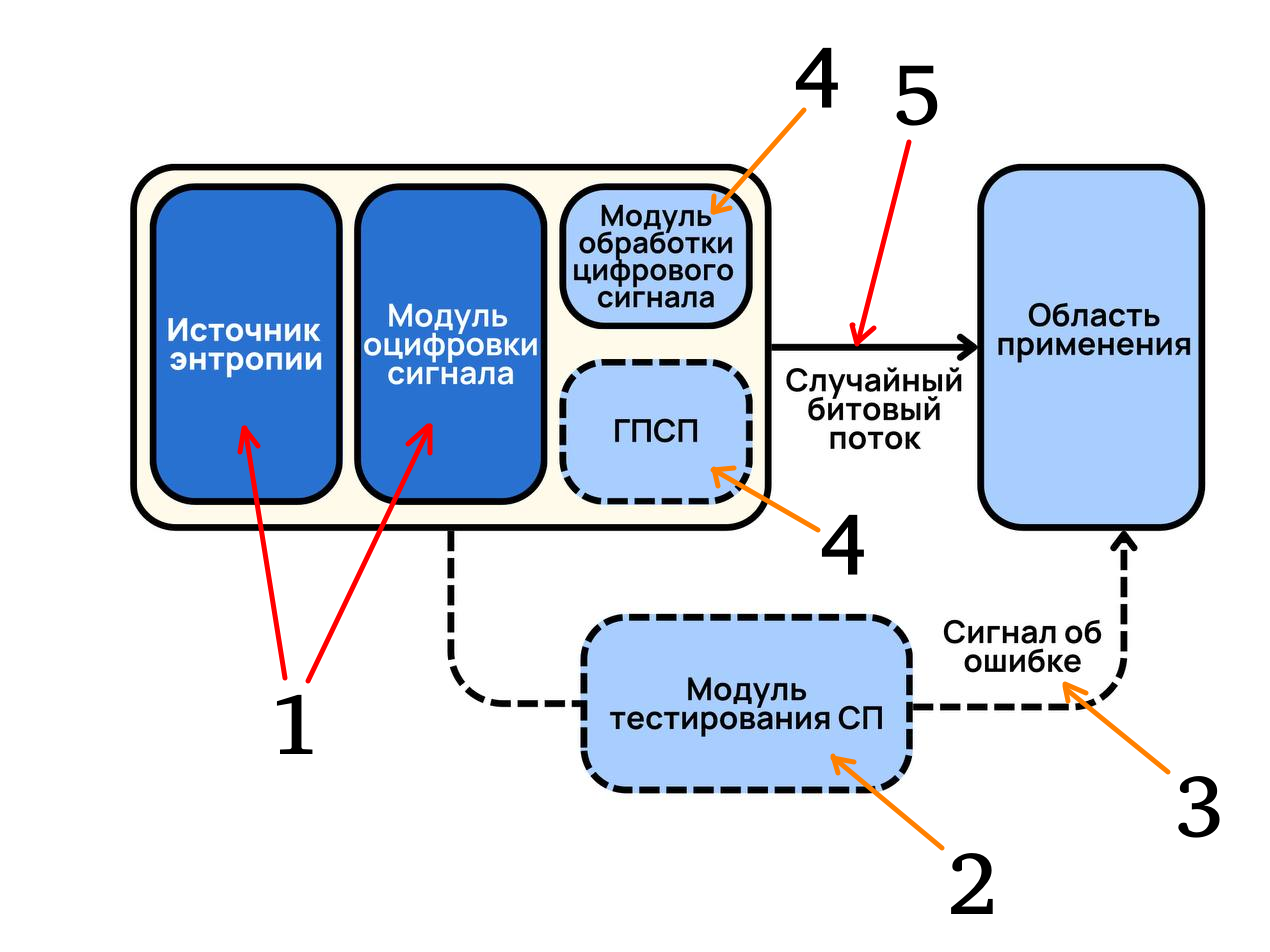
\includegraphics[width=\linewidth,keepaspectratio]{pandoc_media/media/image7.png}

Рисунок 7
\end{minipage}\end{center}

Возможными направлениями для пассивных атак будут: 1, 5. Для активных --
1, 2, 3, 4.

Одним из наиболее изученных классов атак являются атаки через побочные
каналы (SCA, side-channel attacks). Эти методы используют измерения
физических параметров устройства, таких как потребляемая мощность,
электромагнитное излучение, временные задержки или звуковые колебания.
Например, в случае генераторов на основе кольцевых осцилляторов (RO)
было показано, что они уязвимы к активным электромагнитным атакам. При
помощи дифференциального частотного анализа исследователям удалось
извлечь информацию о частотах и расположении осцилляторов. Это, в свою
очередь, позволило провести точную синхронизацию осцилляторов, что
разрушает источник энтропии (джиттер) и делает выход ГИСП предсказуемым.

Другой тип атак -- инъекция ошибок (fault injection) -- предполагает
преднамеренное внесение сбоев в работу схемы. Для этого могут
использоваться такие внешние воздействия, как высокие или экстремально
низкие температуры, мощные электромагнитные поля или интенсивное
освещение. Особенно уязвимы ГИСП на базе свободно работающих
осцилляторов: например, если в питающую цепь подать внешнюю частоту,
можно зафиксировать фазу осцилляции, устранив случайность в выходном
сигнале (Рисунок 8){[}14{]}.

\begin{center}\begin{minipage}{\linewidth}\centering
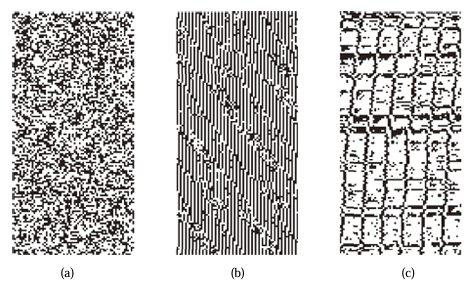
\includegraphics[width=\linewidth,keepaspectratio]{pandoc_media/media/image8.png}

Рисунок 8.
\end{minipage}\end{center}

Атака с использованием частотной инъекции

(a) исходный битовый поток ГИСП (70*140)

(b) инъекция с частотой 1,822880 МГц

(c) инъекция с частотой 1,929629 МГц

Современные достижения в области машинного обучения открыли возможности
для интеллектуальных атак на ГИСП. Одно из исследований
продемонстрировало, что, модифицируя битстрим FPGA-реализации ГИСП
(добавляя сотни дополнительных триггеров), можно обучить модель
глубокого обучения распознавать шаблоны в распределении потребляемой
мощности. Хотя такая атака требует внедрения стороннего кода и потому не
считается полной компрометацией, она подчёркивает потенциальную
опасность аппаратных троянов и направленных ML-атак в будущем.

Для защиты от подобных угроз предлагается несколько мер. Во-первых,
важно физически изолировать чувствительные компоненты ГИСП, например,
размещать развязывающие конденсаторы рядом с кольцевыми осцилляторами.
Во-вторых, структура самого ГИСП должна быть оптимизирована для
устойчивости к внешним воздействиям. Наконец, критически важно внедрение
онлайн-механизмов самотестирования, способных в реальном времени
отслеживать и сигнализировать о любых аномалиях в поведении генератора.

Таким образом, надёжность ГИСП определяется не только качеством
источника энтропии, но и устойчивостью ко множеству атак. Это требует
системного подхода к проектированию и постоянного контроля за состоянием
генератора в процессе эксплуатации.

